\documentclass[12pt]{article}

\usepackage{tabularx}
\usepackage{booktabs}
\usepackage{graphicx}
\usepackage{paralist}
\usepackage{listings}
\usepackage{booktabs}
\usepackage{hyperref}
\usepackage{amsfonts}
\usepackage{amsmath}
\usepackage{color}
\usepackage{fancyhdr}
\usepackage{geometry}
\usepackage{soul}
\usepackage{multirow}
\usepackage{ulem}
\geometry{margin = 0.75in}
\title{SE 3XA3: SRS}

\begin{document}

\maketitle

%%%%%%%%%%%%%%%%%%%Team Information%%%%%%%%%%%%%%%%%%%%%%
{\Large Team Information:}
\begin{table}[htp]
\centering
{\Large
\begin{tabular}{|c|c|c|}
\hline
\multicolumn{1}{|l|}{Team Number} & Name         & MACID   \\ \hline
\multirow{3}{*}{L03 G07}          & Qianlin Chen & chenq84 \\ \cline{2-3} 
                                  & Jiacheng Wu  & wuj187  \\ \cline{2-3} 
                                  & Tingyu Shi   & shit19  \\ \hline
\end{tabular}
}
\end{table}

%%%%%%%%%%%%%%%%%%%%%%%%%%%%%%%%%%%%%%%%%%%%%%%%%%%%%%
\newpage
\begin{table}[htp]
\caption{Revision History} 
\begin{tabularx}{\textwidth}{llX}
\toprule
\textbf{Date} & \textbf{Developer(s)} & \textbf{Change}\\
\midrule
January 26, 2022 & All team members & Initial Document\\
February 9, 2022 & Qianlin Chen & Functional Requirements\\
February 10, 2022 & Jiacheng Wu & Nonfunctional Requirements, Project Drivers, Project Constraints\\
February 10, 2022 & Tingyu Shi & Nonfunctional Requirements, Project Issues\\
April 8, 2022 & All team members & \textcolor{red}{Revise Document}\\
\bottomrule
\end{tabularx}
\end{table}
\newpage
%%%%%%%%%%%%%%Contents%%%%%%%%%%%%%%%%
\tableofcontents
\listoftables
\listoffigures
\cleardoublepage
%%%%%%%%%%% Project Drivers%%%%%%%%%%%%
\section{Project Drivers}
\subsection{The purpose of the Project}
\subsubsection{The User Business or Background of the Project Effort}
Space Invaders is a popular game on the internet and the
corresponding open source project is also loved by people on GitHub. We see the potential of this game and we found that there are some improvements can be done with this game. If we change some outdated features of this game, it should be really fun. After our project is delivered, players can
have better experience with the new version of Space Invaders game.
\subsubsection{Goals of the Project}
This project is to redevelop a game called Space Invaders with
some new features. The aim of this project is to produce an
interesting, addictive and multi-player aircraft shooting game
with a good graphic quality. We expect a service goal that over 80
\% of the players will rate this game over 3/5. Another goal is
to practice software engineering principles during the 
process of development.
\subsection{Stakeholders}
\subsubsection{The Client}
The clients of this project are Dr. Asghar Bokhari and TAs for
course 3XA3. The clients want to redevelop this game since
they 
want to add some features to this game and let developers to
practice software engineering principles. Dr. Asghar Bokhari and TAs will evaluate the delivery of final product and the
process of development.
\subsubsection{The Customer}
The customers of this project are the players who are interested in playing game Space Invaders. As long as 
players can meet the software and hardware requirements, for
example, using Windows, MacOS or Linux, then he or she can be the
customer.
\subsubsection{Other Stakeholders}
\begin{itemize}
\item Members of group 7 are stakeholders of this project. 
Team members will be responsible for writing documents, 
designing modules, implementing and testing.
\item Other software developers are also stakeholders since
this project is public on GitLab and other software
engineers can also redevelop it.
\end{itemize}
\subsection{Users of the Product}
\subsubsection{The Hands-On Users of the Product}
This game is for anyone who knows the basic knowledge of how to operate personal computers. The player’s role is to give input to manipulate the aircraft to move or attack. The way to give input is by pressing the keyboard. This game is suitable for people from all different age groups.
\subsubsection{Priorities Assigned to Users}
\begin{itemize}
\item Key users: The oriented audience of the game are video game lovers  who want to spend time playing video games.
\item Secondary users: Students who want to kill time playing games or learn to do a project of a simple game.
\item Unimportant users: Kids under 12 who want to gain hand-eye coordination and problem solving skills.
\end{itemize}
\subsubsection{User Participation}
The players should spend at least 10 mins on this game and shall have basic knowledge of operating the computers. We want to
hear the advice from users about the following perspective:
\begin{itemize}
\item Graphic Design
\item Difficulty level of this game (We do not want our game
to be too difficult to make players lose interests to play it)
\item Game Items design
\item Overall experience
\end{itemize}
\section{Project Constraints}
\subsection{Mandated Constraints}
\subsubsection{Solution Constraints}
\begin{itemize}
\item The project will be implemented by python since the old version is done by python. It is time saving to do it in python.
\item Pygame library will be used in implementation since it
is a suitable library to use for game development in python.
\item The solution must follow proper software engineering
principles.
\end{itemize}
\subsubsection{Implementation Environment of the Current System}
The project will be done in Windows and Linux(MacOS), which means the product will be able to run on those environments.
\subsubsection{Partner or Collaboration Applications}
N/A
\subsubsection{Off-the-Shelf Software}
N/A
\subsubsection{Anticipated Workplace Environment}
N/A
\subsubsection{Schedule Constraints}
The first version of project must be finished before Mar 22, 2022 because the project will be first demonstrated on that day. The final product should be done before April 12, 2022.
\subsubsection{Budge Constraints}
N/A
\subsection{Naming Conventions and Definitions}
\begin{itemize}
\item Aircraft: A player will control the aircraft to play the game. The player will give inputs to system to manipulate the aircraft and the aircraft will react accordingly.
\item Monster: Monsters are the opponents(bad guys) of players. A player has to eliminate all of the monsters 
in order to win the game.
\item Health points: It stands for the health of the aircraft. The aircraft will lose one health point once it gets hit
by bullets from monsters.
\item Ammo item: If the aircraft shoots an Ammo item, \textcolor{red}{\st{the aircraft's ammo type will be upgraded to a more powerful one.} the system will 
allow the aircraft to shoot one more bullet at the same time.}
\item Health item: If the aircraft shoots a Health item, the aircraft will gain one more health point.
\item Bomb item: If the aircraft shoots a Bomb item, the bomb will explode and do damage to a big range of the area in the
monster matrix.
\end{itemize}
\subsection{Relevant Facts and Assumptions}
\subsubsection{Facts}
\begin{itemize}
\item The original project has 700 lines of code.
\item The original project has soundtracks, but they will be removed because the soundtracks may make people uncomfortable.
\end{itemize}
\subsubsection{Assumptions}
\begin{itemize}
\item Users should have basic equipments to play the game,
including a laptop, a mouse and a keyboard.
\item Users should know how to operate a PC.
\item Users should understand basic English.
\end{itemize}
\newpage
\section{Functional Requirements}
\subsection{The Scope of Work and Product}
\subsubsection{The Context of the Work}
The original Space Invaders has poor implementation documentation and is not a fully functional game platform for the user to interact with to win the game. Not only does Space Invaders fails to deliver a user-friendly game but it also fails to meet the software engineering design principles. Space Invaders is not ideal for a developer to understand the game’s \textcolor{red}{\st{file structure} architecture} \textcolor{red}{\st{and working software}} as it lacks documentation and modular design in the project. Therefore, our new Space Invaders has the following goals: 
\begin{itemize}
\item Redesign the game following software engineering principles and process for the benefit of other developers.
\item Give the user an interactive and engaging game with an understandable winning criteria and functionality
\end{itemize}
The following is a Work Context Diagram:
\begin{figure}[h!]
\begin{center}
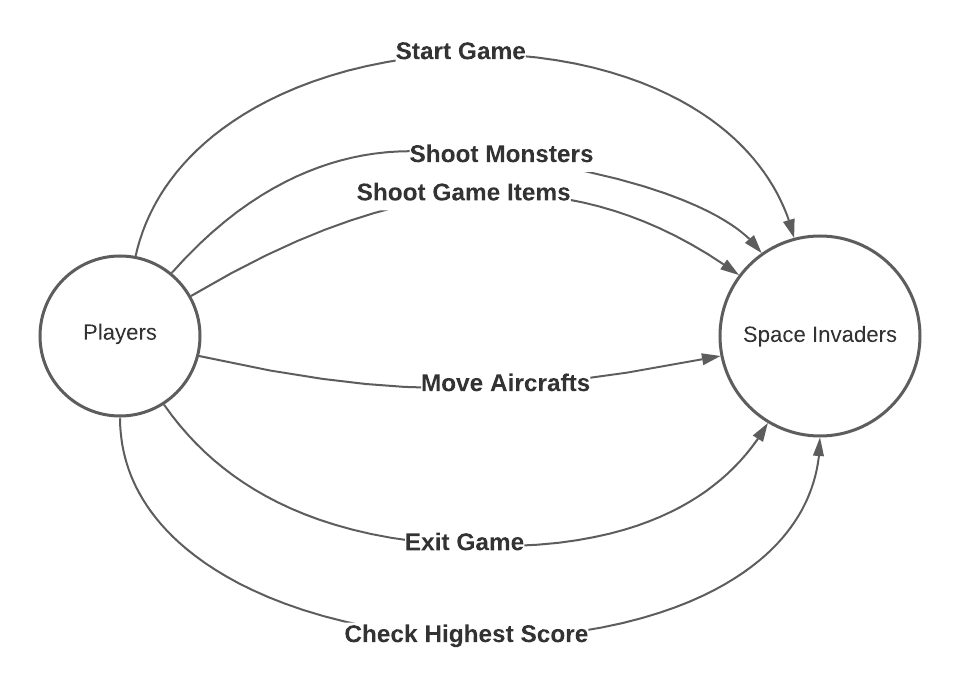
\includegraphics[scale=1]{Context_Diagram.png}
\end{center}
\caption{\textcolor{red}{OLD} Context Diagram}
\end{figure}
\newpage
\begin{figure}[h!]
\begin{center}
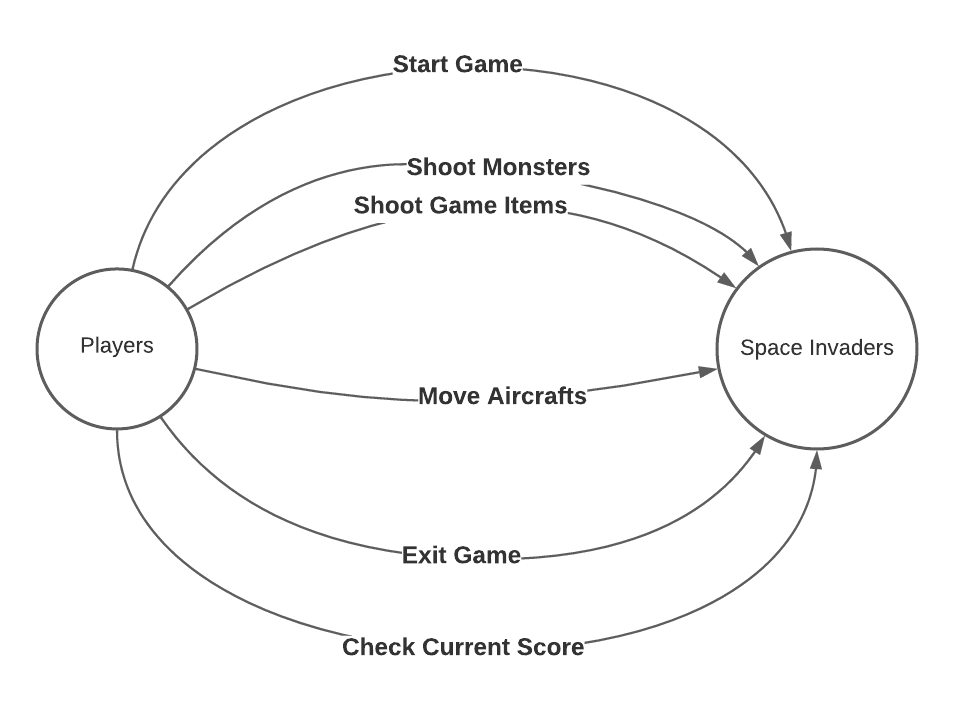
\includegraphics[scale=1]{New_Context_Diagram.png}
\end{center}
\caption{\textcolor{red}{NEW} Context Diagram}
\end{figure}
\newpage
\subsubsection{Work Partitioning}
\begin{table}[h!]
\centering
\begin{tabular}{| p{3.5cm} | p{3cm} | p{3cm}| p{8cm}|}
\hline
\textbf{Business Event} & \textbf{Inputs} & \textbf{Outputs}&\textbf{Summary}\\
\hline
Start Game& Keyboard (Players press \textcolor{red}{\st{any} Enter/Return} key to start) & Display instructions and let players to choose playing mode & 
\begin{itemize}
\item Creates game frame with monsters, game items, aircraft and obstacles.
\item Create five rounds of game
\item Presents two playing modes for players
\item Display game instructions
\end{itemize}
\\
\hline
Shoot Monsters & Keyboard Input & Monster disappears in GUI & Based on the player's actions, aircraft will attack 
monsters which are controlled by the system.\\
\hline
Shoot Game Items & Keyboard Input & Game Items disappear in the monster matrix and display the corresponding changes due to game items & The players can shoot game items inside the
monster matrix.\\
\hline
Move Aircraft & Keyboard Input & Aircraft changes position & 
Different keyboard input will represent aircraft moving left
or right.\\
\hline
Exit Game & Keyboard Input & Exit game window & Players can
exit game by clicking the cross icon on the up right
corner.\\
\hline
Check \textcolor{red}{\st{Highest} current game} Score & N/A & 
Display \textcolor{red}{\st{highest point} current game score} on the screen & Players can 
check the \textcolor{red}{\st{highest score} current game score} on the screen.\\
\hline
\end{tabular}
\caption{Work Partitioning Table}
\end{table}
\newpage
\subsubsection{Individual Project Use Cases}
The following is the use case diagram:
\begin{figure}[h!]
\begin{center}
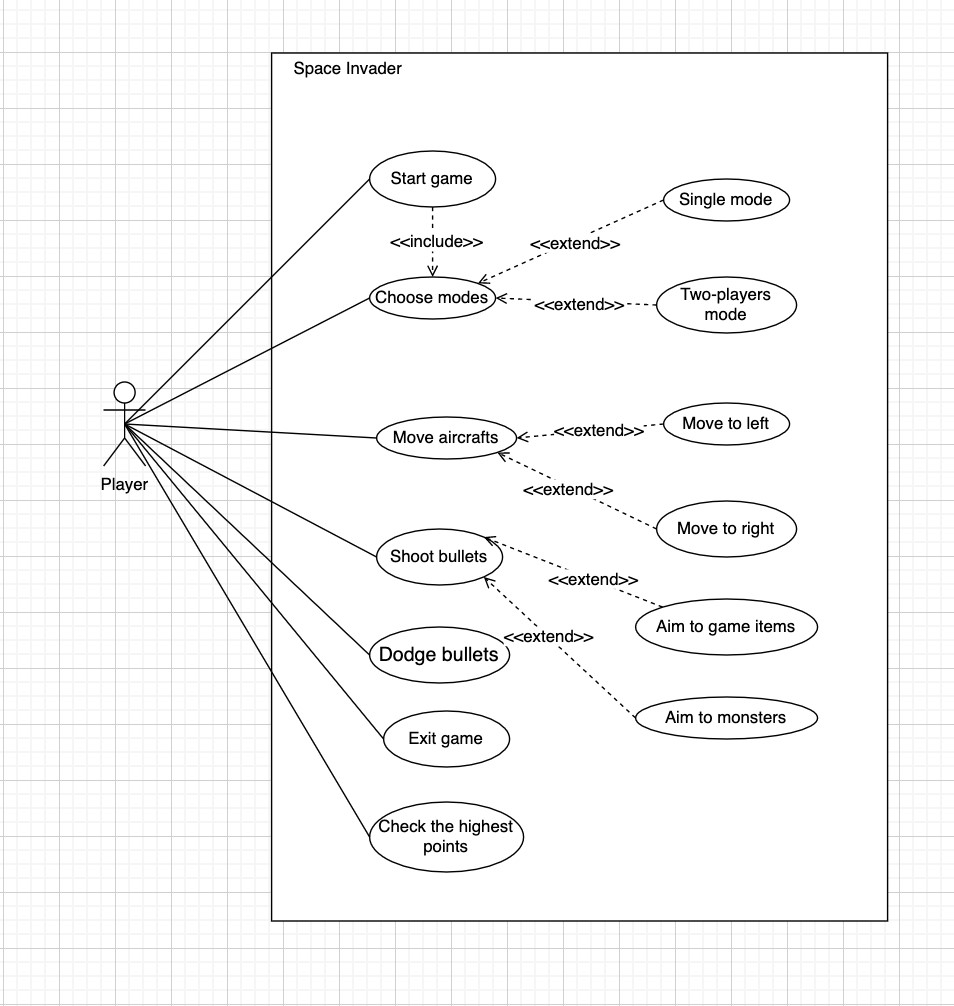
\includegraphics[scale=1]{Use_Case.png}
\end{center}
\caption{\textcolor{red}{OLD} Use Case Diagram}
\end{figure}
\newpage
\begin{figure}[h!]
\begin{center}
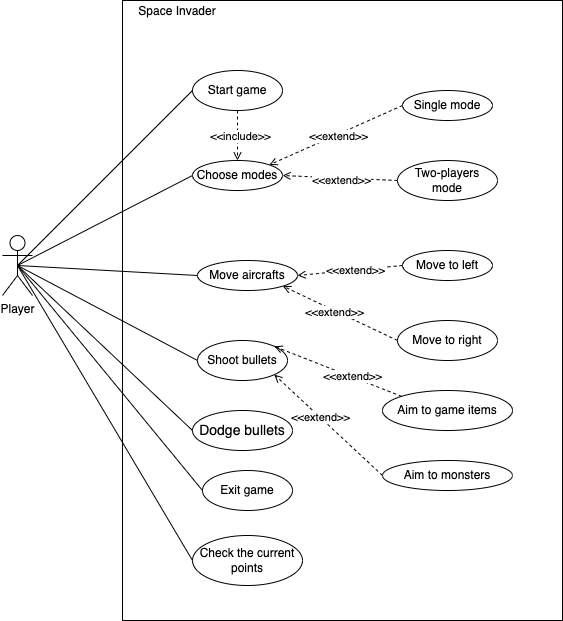
\includegraphics[scale=0.8]{Revised_Use_Case.png}
\end{center}
\caption{\textcolor{red}{NEW} Use Case Diagram}
\end{figure}
\newpage


\subsection{Functional Requirements}
We will state functional requirements from system viewpoint
and user viewpoint perspectives:
\subsubsection{System Viewpoint}
\begin{enumerate}[{FR}1:] 
\item The system shall prompt players to choose single-player
mode or two-players mode.
\item The system shall display the information about monsters’
types \textcolor{red}{\st{ (green, blue and pink)}} and corresponding points \textcolor{red}{\st{(10, 20 and 30)}} at the starting page.
\item The system shall display instructions about how to 
play to game after the starting page.
\item The system shall display the total scores for one player
or two players, and the initial score should be zero.
\item The system shall display the \textcolor{red}{\st{total five}} health points for each player in different modes at the beginning.
\item The system shall display \textcolor{red}{\st{a galaxy picture as}} game background.
\item The system shall display monsters as a matrix for each round \textcolor{red}{\st{(5 rows and 10 columns)}}.
\item The system shall display game items (bomb, ammo and health) randomly inside the monster matrix. For the details of these items, please refer to the naming convention.
\item The system shall display one aircraft in single-player mode and two aircraft in two-player mode.
\item The system shall display \textcolor{red}{\st{four}} obstacles between the aircraft and monsters.
\item The system shall display the final score at the termination of game.
\item The system shall display ‘WIN!’ once players pass five rounds.
\item The system shall display ‘FAIL’ in following situations:
\begin{itemize}
\item In single-player mode: The only one player loses five health points.
\item In two-players mode: Both players lose five health points.
\end{itemize}
\item \textcolor{red}{\sout{ The system shall display back to starting page after displaying ‘WIN!’ or ‘FAIL’ for allowing players to replay.}}
\item The system shall increase players’ total scores once they hit the monsters.
\item The system shall increase players’ total health points when they hit the health item and decrease health points when players’ aircraft are shot by monsters.
\item \textcolor{red}{\sout{The game shall contain 5 rounds.}}
\item \textcolor{red}{The game shall contain 5 rounds with different patterns of monster matrix. \sout{The game shall set five rows of green monsters in round 1.} }
\item \textcolor{red}{\sout{The game shall set three rows of green monsters and two rows of blue monsters in round 2.}}
\item \textcolor{red}{\sout{The game shall set five rows of blue monsters in round 3.}}
\item \textcolor{red}{\sout{The game shall set one row of green monsters, three rows of blue monsters and one row of pink monsters in round 4.}} 
\item \textcolor{red}{\sout{The game shall set five rows of pink monsters in round 5.}}
\item The system shall set monsters’ movement be east-south-west under a constant velocity.
\item The system shall let monsters shoot bullets randomly.
\item The system shall let green monsters die after being shot once (from players’ aricraft).
\item The system shall let blue monsters die after being shot twice (from players’ aircraft).
\item The system shall let pink monsters die after being shot three times (from players’ aircraft).
\item The system shall let a monster disappear if it dies.
\item The system shall reduce the area of obstacles if they are shot by monsters or aircraft.
\item The system shall set game items in a way that they can only be obtained by aircraft’s bullets instead of monsters’ bullets.
\item The system shall limit the amount of game items for each round.
\item The system shall provide bombs which can destroy \textcolor{red}{four random monsters inside the matrix \sout{the monsters around it (8 in total)}} once it is shot by aircraft.
\item The system shall provide ammo game items to increase the number of aircraft bullets by 1.\textcolor{red}{\sout{ only for the present round}}. 
\item The system shall provide heart to increase aricraft's health points by one once it is shot by aircraft.
\item[FR35] The system shall have random occurrence for each game item.
\end{enumerate}

The following are some summaries about Functional requirements from system viewpoint:
\begin{itemize}
\item FR17 - FR21 describes how to set up 
monster matrix for each round.
\item FR22 - FR27 describes monsters' behaviors.
\item FR30 - FR35 describes game items.
\end{itemize}
\subsubsection{User Viewpoint}
\begin{enumerate}
\item [FR36:]The game shall be able to start by \textcolor{red}{\st{entering any keys.} pressing Enter/Return}
\item [FR37:]The system shall be able to exit any time by clicking cross icon. \textcolor{red}{\st{at up right corner.}}
\item [FR38:]The system shall allow the player to move the aircraft left or right by operating keyboards. \textcolor{red}{\st{by clicking $\leftarrow$ or $\rightarrow$ in 
the single-player mode.}}
\item[FR39:] \textcolor{red}{\st{The system shall allow player A to move the aircrafe left or right by click $\leftarrow$ or $\rightarrow$ and let player B
to move left or right by clicking A or
D in the two-players mode.}}
\item [FR40:]The system shall let each player shoot the monsters by one bullet as default.
\end{enumerate}
\section{Nonfunctional Requirements}
\subsection{Look and Feel Requirements}
\subsubsection{Appearance Requirements}
\begin{itemize}
\item[NFR1:] The product shall have a good graphic quality.\\
Fit Criterion: FPS of the product shall be over 30 fps and the graphics should be over 8 bit.
\item[NFR2:] The product shall display all the \textcolor{red}{\st{elements in game} game elements} clearly enough to recognize.\\
Fit Criterion: 8 out of 10 random persons can recognize all the elements directly.
\end{itemize}
\subsubsection{Style Requirements}
\begin{itemize}
\item[NFR3:] The game display should follow the style of minimalism.\\ Fit Criterion:
\textcolor{red}{8 out of 10 random persons should think that the game display follows
the style of minimalism.}
\item[NFR4:] The mood of the graphics should be intense.\\Fit Criterion:
\textcolor{red}{8 out of 10 random persons should think the mood of graphics is intense.}
\end{itemize}
\subsection{Usability and Humanity Requirements}
\subsubsection{Ease of Use Requirements}
\begin{itemize}
\item[NFR5:]The product shall be easy for a 10-year-old child to operate.\\
Fit Criterion:Over 8 out 10 10-year old children assess this game as easy.
\item[NFR6]: The product shall be used by people with no training.\\
Fit Criterion:Over 8 out 10 people with no training know how to play this game after 5 minutes of learning.
\end{itemize}
\subsubsection{Personalization and Internationalization Requirements}
N/A
\subsubsection{Learning Requirements}
\begin{itemize}
\item[NFR7:] The product shall allow users to understand all the rules of the game quickly.\\
Fit Criterion: All sample users can learn all the rules of the game in 10 minutes.
\end{itemize}
\subsubsection{Understandability and Politeness Requirements}
N/A
\subsubsection{Accessibility Requirements}
N/A
\subsection{Performance Requirements}
\subsubsection{Speed and Latency Requirements}
\begin{itemize}
\item[NFR8:] In selection menu interface, The system shall respond user inputs quickly.\\
Fit Criterion: In selection menu interface, the system shall respond user inputs within 1 second.
\end{itemize}
\subsubsection{Safety-Critical Requirements}
N/A
\subsubsection{Precision of Accuracy Requirements}
\begin{itemize}
\item[NFR9:] In gaming interface, the system shall respond to user operating inputs quickly.\\
Fit Criterion: In gaming interface, the system shall respond user operating inputs within 1 second.
\end{itemize}
\subsubsection{Reliability and Availability Requirements}
\begin{itemize}
\item[NFR10:] The product shall be available for long-term use. \\
Fit Criterion: The product shall be available for 24 hours per day, 365 days per year.
\end{itemize}
\subsubsection{Robustness and Fault-Tolerance Requirements}
N/A
\subsubsection{Capacity Requirements}
\begin{itemize}
\item[NFR11:] The product shall run steadily when in two-players mode.\\
Fit Criterion: In two-players mode, the game runs normally for at least 2 hours.
\end{itemize}
\subsubsection{Scalability or Extensibility Requirements}
N/A
\subsubsection{Longevity Requirements}
N/A
\subsection{Oerational and Environment Requirements}
\subsubsection{Expected Physical Environment}
\begin{itemize}
\item[NFR12:] The product shall run on regular PCs.\\ Fit Criterion: The game should run on different operating systems
correctly 9 times out of 10.
\end{itemize}
\subsubsection{Requirements for Interfacing with Adjacent Systems}
\begin{itemize}
\item[NFR13:] The product shall run without errors on the most popular operating systems.\\
Fit Criterion: The product can run normally on Windows, Linux and MacOS.
\end{itemize}
\subsubsection{Productization Requirements}
\begin{itemize}
\item[NFR14:] \textcolor{red}{\st{The product shall be distributed as a EXE file. \\ Fit Criterion: N/A}}
\item[NFR15:] The product shall be installed by an untrained user without complex instructions.\\
Fit Criterion: 8 out of 10 untrained users can install the game without any trouble.
\end{itemize}
\subsubsection{Release Requirements}
N/A
\subsection{Maintainability and Support Requirements}
\subsubsection{Maintenance Requirements}
\begin{itemize}
\item [NFR16:]For any new features to be added, the implementation should be finished as soon as possible.\\ Fit Criterion: The MIS should be ready within one week since 
adding new features decisions are made. After that, coding
and testing should be completed within one week. Given the size
of our project, this timeline is feasible.
\item[NFR17:] All the code should be well documented. \\ Fit Criterion: The code should be documented using doxygen.
\end{itemize}
\subsubsection{Supportability Requirements}
\begin{itemize}
\item[NFR18:] There must be a way that developers can 
communicate with players so that developers can receive the
advice from players and offer support to players.\\Fit Criterion: The repo of this game should remain public so that
developers and players can communicate via GitLab.
\end{itemize}
\subsubsection{Adaptability}
\begin{enumerate}
\item[NFR19:] The product is expected to run under 
different operating systems. \\ Fit Criterion: The game should
be able to be executed in Windows, Linux and MacOS.
\end{enumerate}
\subsection{Security Requirements}
\subsubsection{Access Requirements}
\begin{itemize}
\item[NFR20:] In two-players mode, player A can not have
control of player B's aircraft and vice versa.\\Fit Criterion
:The control modules of two aircraft should be separated in
module design.
\end{itemize}
\subsubsection{Integrity Requirements}
\begin{itemize}
\item[NRF21:]\textcolor{red}{\st{This game can record the highest score and 
players can not access to this file.\\Fit Criterion: Highest
score should be private so that it is inaccessible from outside.}}
\end{itemize}
\subsubsection{Privacy Requirements}
N/A
\subsubsection{Audit Requirements}
N/A
\subsubsection{Immunity Requirements}
N/A
\subsection{Cultural and Political Requirements}
\subsubsection{Cultural Requirements}
\begin{itemize}
\item[NFR22:]The game shall not contain any offensive contents
to religious and ethnic groups. \\Fit Criterion: This game 
will not contain many words, therefore, developers should be
carefully about pictures used in GUI.
\end{itemize}
\subsubsection{Political Requirements}
N/A
\subsection{Legal Requirements}
\subsubsection{Compliance Requirements}
\begin{itemize}
\item[NFR23:]The system shall not break and Canadian Laws. \\Fit Criterion: 
\textcolor{red}{Game should be approved by some law institution.}
\end{itemize}
\subsubsection{Standards Requirements}
N/A
\subsection{Health and Safety Requirements}
\begin{itemize}
\item[NFR24:] \textcolor{red}{\st{The game developers shall notify players to 
avoid game addiction.\\Fit Criterion: Game shall display a message after the starting
page to tell players to avoid game addiction.}}
\end{itemize}
\newpage
\section{Project Issues}
\subsection{Open Issues}
\begin{enumerate}[{Issue}1.]
\item The original project has all the code written in just 
one \verb|.py| file. The issue is to redesign the modules to
achieve software engineering principles.
\item Our team hopes that executable file can be executed on
Windows, Linux and MacOS. We are still looking for ways to 
create executable files for MacOS and Linux.
\item Since this game includes GUI, our team is still thinking
about appreciate ways to test GUI.
\end{enumerate}
\subsection{Off-the-Shelf Solutions}
\subsubsection{Ready-Made-Product}
Since our new Space Invaders game has some new features
and  will
be developed using proper software principles, we can not
find any existing solutions.
\subsubsection{Reusable Components}
\verb|Pygame| library can be used for implementing games in python.
For testing, we can use \verb|Pytest| and \verb|unittest|
libraries.
\subsubsection{Products That Can Be Copied}
The original project is a similar product. This is the \href{https://github.com/leerob/space-invaders}{\textcolor{red}{Link}}.\\
\subsection{New Problems}
\subsubsection{Effects on the Current Environment}
The new product will not affect the current implementation
environment. However, our product should not do the following 
things:
\begin{itemize}
\item Bring Malware software to players' computers.
\item Use too much computer resources when running.
\end{itemize}
\subsubsection{Effects on the Installed Systems}
If the user wants to run the source code to play the game, then required 
libraries should be installed first.
\subsubsection{Potential User Problems}
N/A
\subsubsection{Limitations in the Anticipated Implementation Environment That May Inhibit the New Product}
N/A
\subsubsection{Follow-Up Problems}
N/A
\subsection{Tasks}
\subsubsection{Project Planning}
The project schedule is created as a Gantt Chart which can
be found using this \href{https://gitlab.cas.mcmaster.ca/shit19/2022_winter_3xa3_l03_g07/-/tree/main/ProjectSchedule}{\textcolor{red}{Link}}
\subsubsection{Planning of the Development Phases}
\begin{enumerate}[{Phase}1:]
\item Listing all the functional and nonfunctional requirements. Phase 1 has already finished in this document.
\item After having all the requirements, phase 2 will be
designing modules and module interfaces.
\item Coding according to MG and MIS developed in phase 2.
\item Testing the final product.
\end{enumerate}
\subsection{Migration to the New Product}
Our project is independent from the original project, there 
are no requirements for Migration to the New Product.
\subsection{Risks}
The following are some risks with this project:
\begin{enumerate}[{R}1:]
\item Implementation Difficulties: \\This game will be implemented with python.
The good news is that every team member has
experience with this language. However, we need to use pygame module for implementation and only one team member has experience with this module. Therefore, other two team members should spend time to learn this module and familiarize with the API.
\item Testing:\\ Game testing is usually harder compared with
testing of other projects. The main difficulty here is to choose an appropriate
testing method so that it can cover all the scenarios.
\item Portability:\\
We believe that source code can be executed
in different operating systems. However, the
problem is to make sure that executable files
can be executed in different operating systems.
\newpage
\item Design and Requirements Difficulties:
\begin{itemize}
\item Design Difficulty: The main difficulty in design process is designing appropriate modules. We need to make sure 
that each module is low coupling and high cohesion.
\item Requirements Difficulty: The main difficulty for requirements engineering is 
to solve conflicts and make sure the final
requirements document does not have any conflicts. 
\end{itemize}
\end{enumerate}
\subsection{Costs}
This project is based on an open project and all the libraries
are free to use, so this project does not involve monetary cost. However, there are time costs, minimum 4 hours of 
weekly meeting are needed.
\subsection{User Documentation and Training}
\subsubsection{Documentation}
After the starting the page, there will be a page to show
instructions of how to play the game.
\subsubsection{Training}
This game is quit easy to learning. No training is required.
\subsection{Waiting Room}
The following are some potential future features:
\begin{itemize}
\item  The system shall allow two players to connect and play
two-player mode via internet.
\item Add more interesting game items.
\item Introduce game currency. Maybe players can buy aircraft
skins using the currency.  
\end{itemize}
\subsection{Ideas for Solutions}
The following are some potential modules for the game 
implementation, this may change during the design process:
\begin{itemize}
\item Single Player Mode
\item Two Players Mode
\item Monster Matrix
\item Aircraft
\item Game items
\item Obstacles
\item Record Highest Score
\item bullets
\item Health Points
\end{itemize}
\section{Reference}
Robertson, James, and Suzanne Robertson. "Volere." Requirements Specification Templates (2000).
\end {document}
